% !TeX spellcheck = en_US
\documentclass[12pt,svgnames,table,draft=false]{beamer}

\usefonttheme{structurebold}

\usepackage[utf8]{inputenc}
\usepackage{framed}
\usepackage[caption=false]{subfig}
\usepackage{tcolorbox}
%\setbeamertemplate{caption}[numbered]
%\setbeamertemplate{blocks}[rounded][shadow=false]
%\setbeamercovered{invisible}
\setbeamertemplate{caption}[numbered]

\usepackage{graphicx}
\usepackage{tikz}
\usepackage{epstopdf}
\usepackage{import}
\usepackage{footbib}
\usepackage[absolute]{textpos}
% \usepackage[style=numeric-comp, backend=bibtex]{biblatex}

\newcommand{\mbf}[1]{\mathbf{#1}}
\graphicspath{ 
{../../images/}
}

\newcommand{\Htwo}{\ensuremath{\textrm{H}_2} }
\newcommand{\Hinf}{\ensuremath{\textrm{H}_\infty} }
\newcommand{\Mu}{\ensuremath{\mu} \,}
\providecommand{\mbf}[1]{\mathbf{#1}}
\newcommand{\idxFollower}{{\ensuremath{i} }}
\newcommand{\idxPredecessor}{{\ensuremath{i-1} }}
\newcommand{\idxSample}{{\ensuremath{k}}}
\newcommand{\idxAxis}{{\ensuremath{p}}}
\newcommand{\Francois}{\mbox{Fran\c{c}ois Defa$\ddot{\textrm{y}}$}}
  
\addtobeamertemplate{navigation symbols}{}{%
    \usebeamerfont{footline}%
    \usebeamercolor[fg]{footline}%
    \hspace{1em}%
    \insertframenumber/\inserttotalframenumber
}

\begin{document}
\usebackgroundtemplate{
%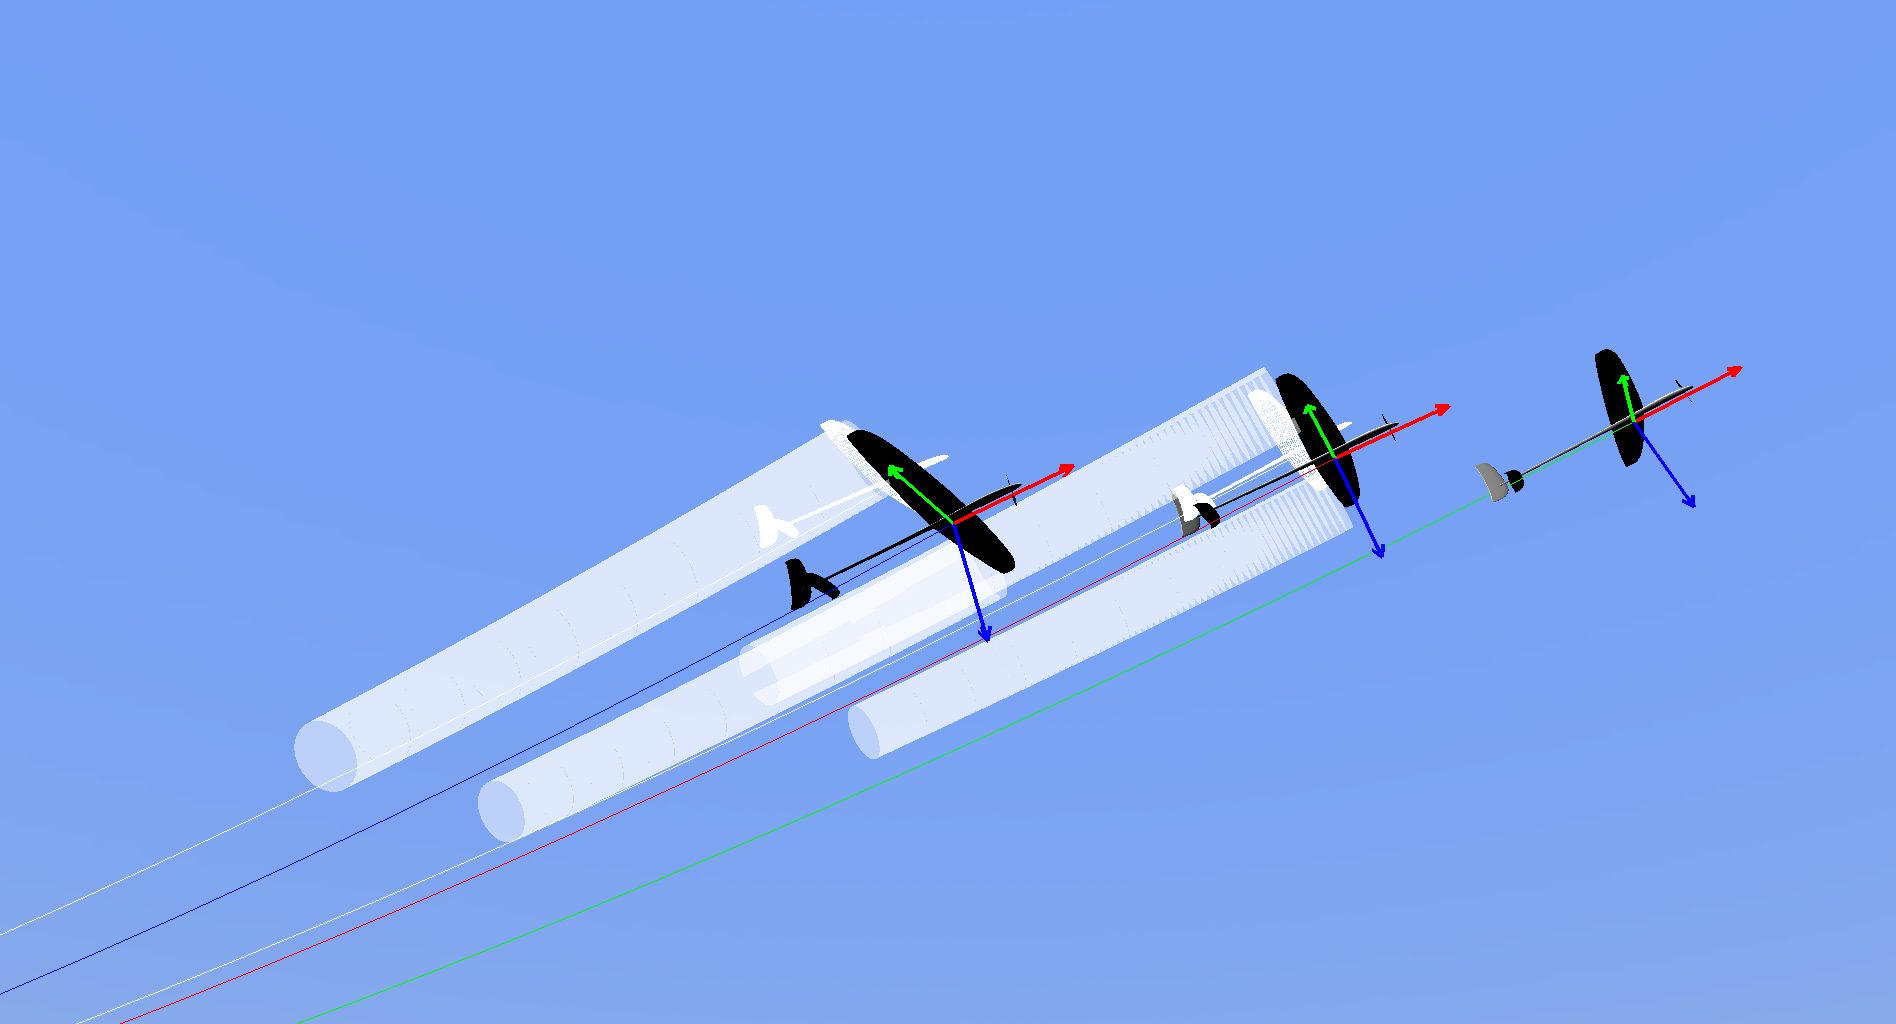
\includegraphics[width=\paperwidth,height=\paperheight]{UAV3D_N=2_sky}
}

\title{Discrete Sliding Mode control of small UAS in tight formation flight under information constraints}

\author{J.Bolting\inst{1} \and S.Fergani\inst{1} \and J.-M.Biannic\inst{2} \and F.Defay\inst{1} \and M.Stolle\inst{2}}
  
\institute[VFU] % (optional)
{
\inst{1}Institut Supérieur de l'Aéronautique et de l'Espace (ISAE)  
\and
\inst{2}Office National d'Études et de Recherches Aérospatiales (ONERA) 
}
 
\date{IFAC ACA'16}

\maketitle

\usebackgroundtemplate{}

\begin{frame}{Outline}
  $\Rightarrow$ Motivation\\
  \vspace{1em}
  $\Rightarrow$ Challenges \\
  \vspace{1em}
  $\Rightarrow$ Sliding Mode Control for relative position holding\\
  \vspace{1em}  
  $\Rightarrow$ Predictive Discrete Sliding Mode Guidance laws \\
  \vspace{1em}  
  $\Rightarrow$ Overview \\
\end{frame}

\usebackgroundtemplate{
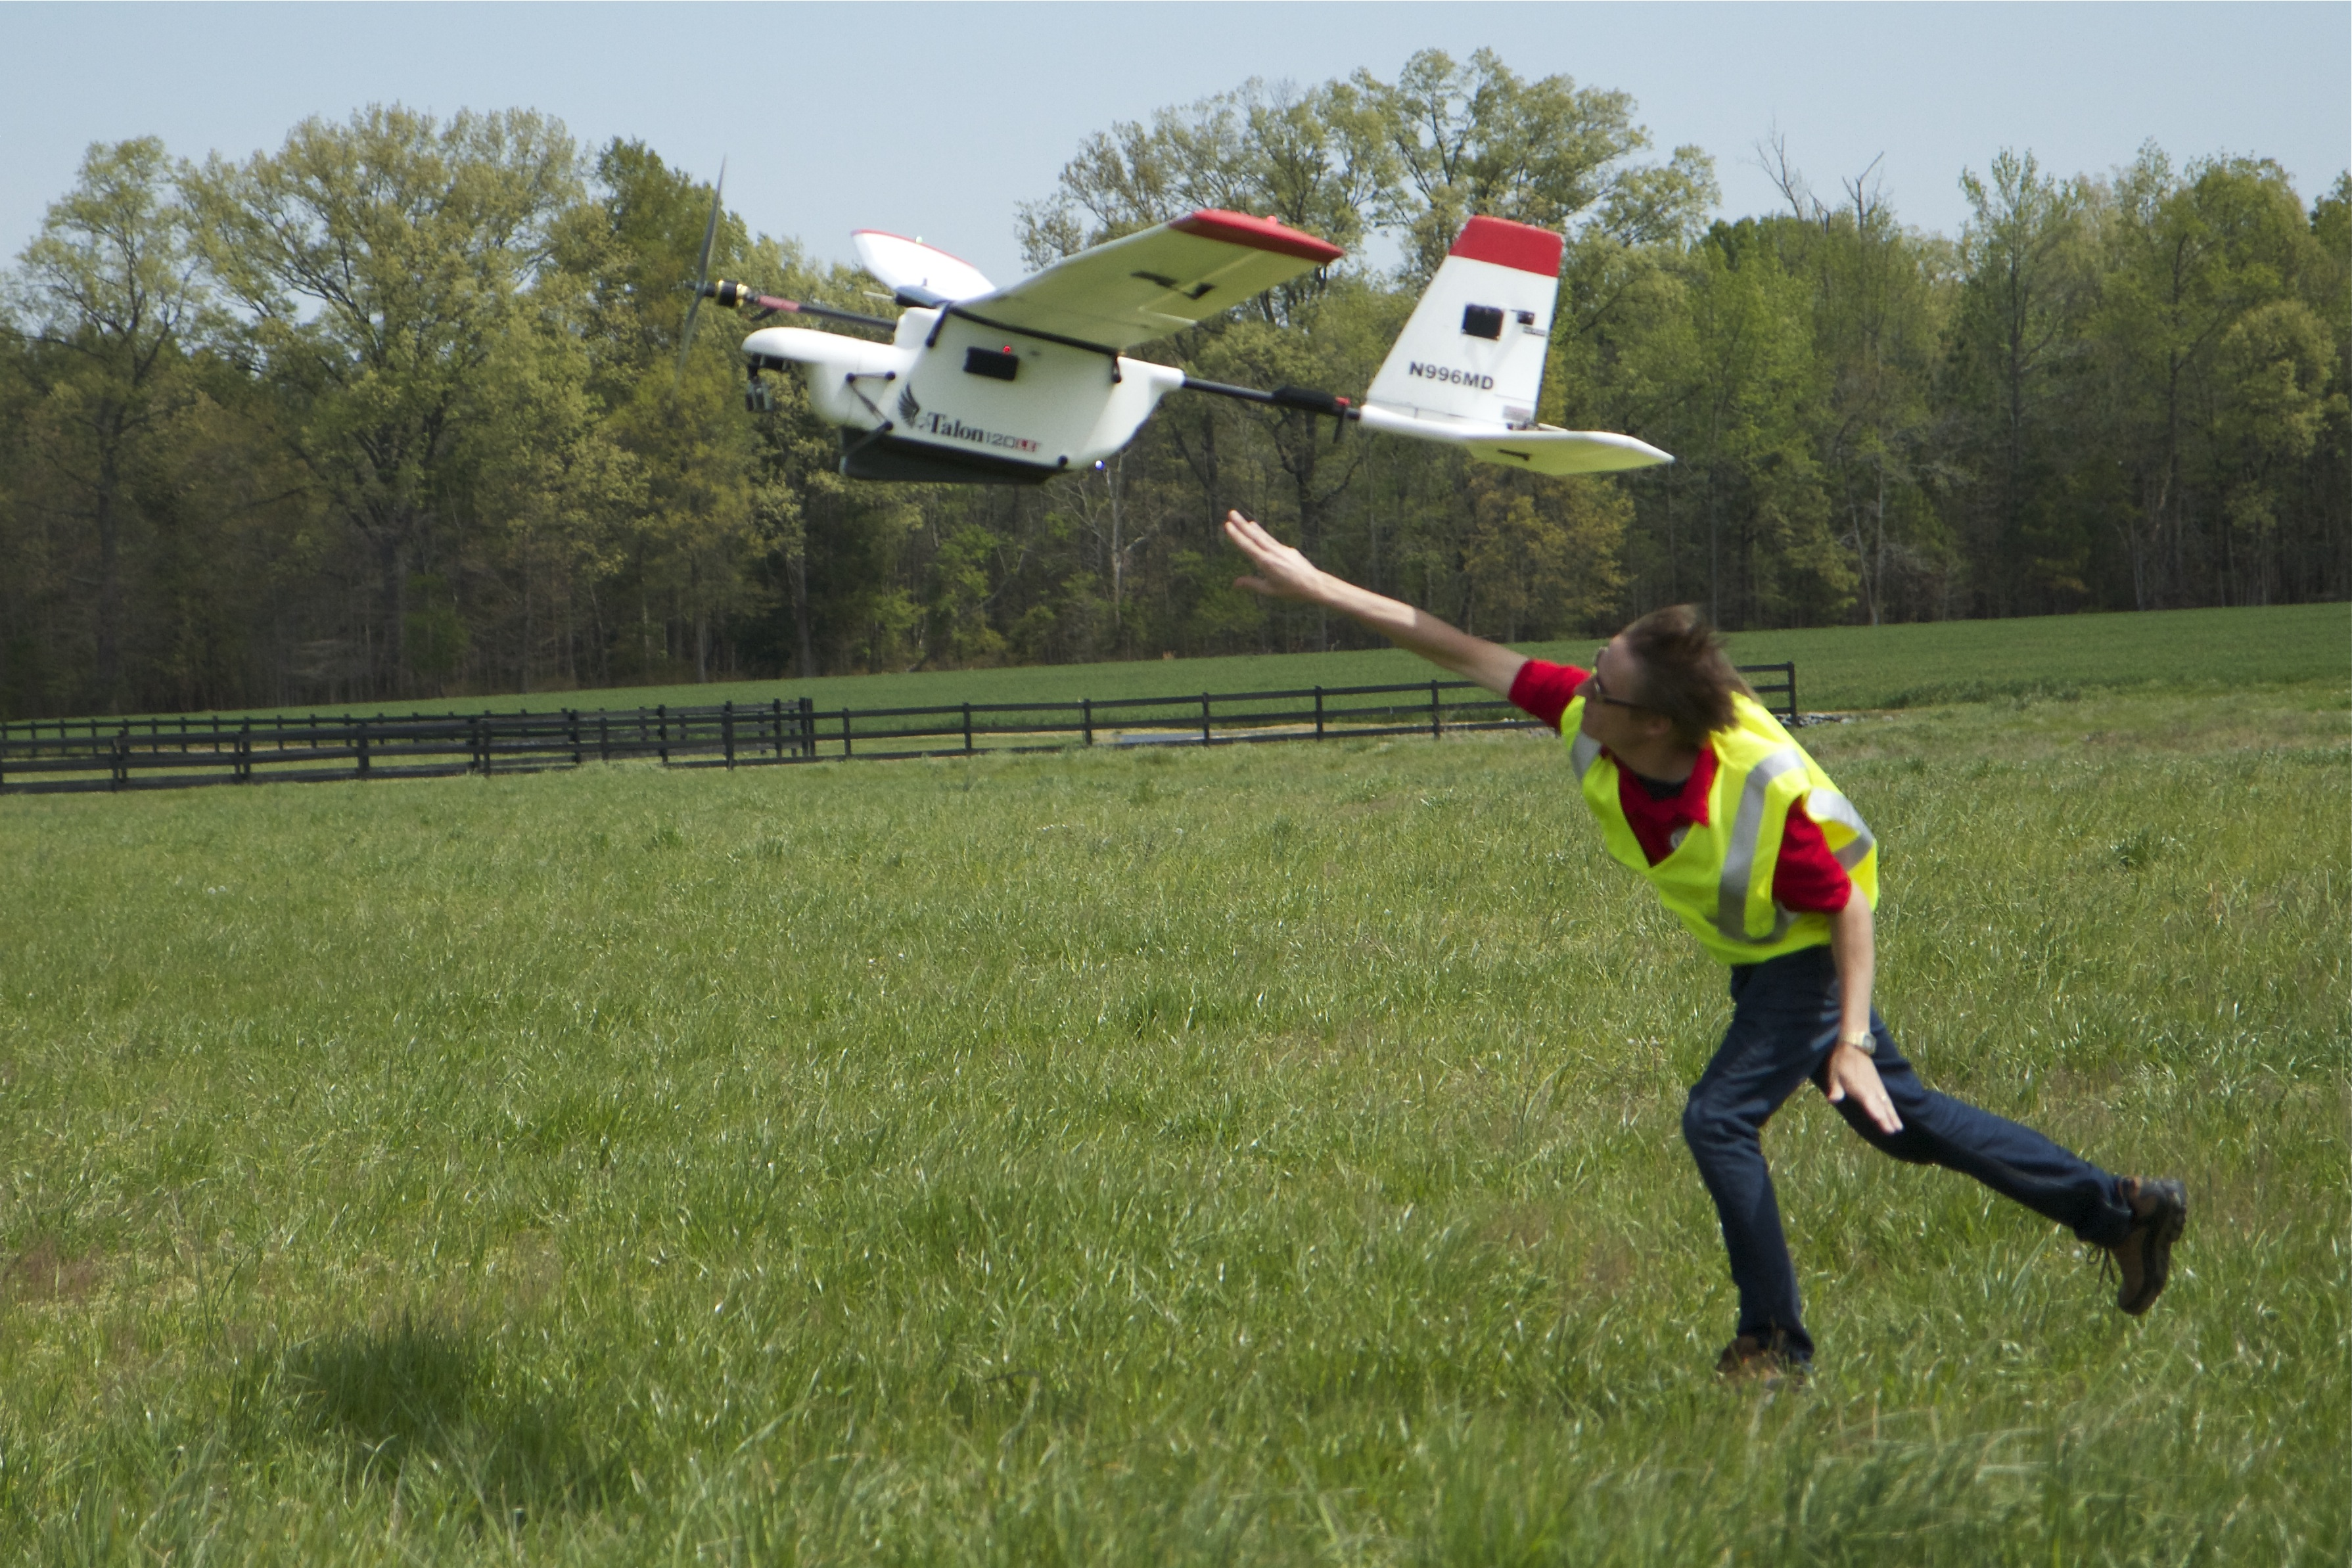
\includegraphics[width=\paperwidth,height=\paperheight]{UAV-javelinlaunch}
}
\begin{frame}{+}
\vspace{7em}
\centering
	\begin{tcolorbox}[width=.8\textwidth,colback={gray!10!}]  
	\centering
	\Large
	Small UAS \\
	= \\
	Inexpensive \\
	Easy to operate
	\end{tcolorbox}  
	
\end{frame}


\usebackgroundtemplate{
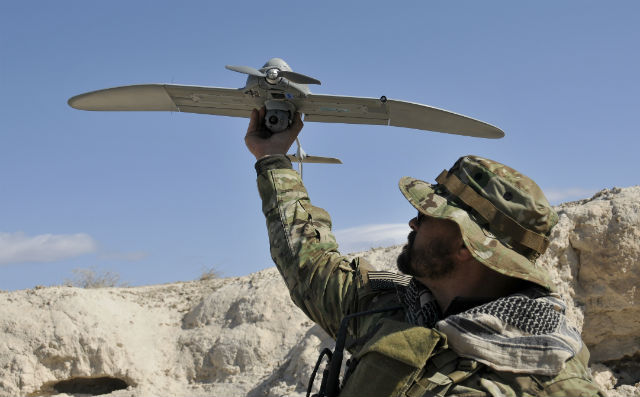
\includegraphics[width=\paperwidth,height=\paperheight]{wasp_launch}
}
\begin{frame}{-}
	\centering
	\vspace{+5em}
	\begin{tcolorbox}[width=.8\textwidth,colback={gray!10!}]  
	\centering
	\Large
	Small UAS \\
	= \\
	Small payload  \\
	Small endurance 
	\end{tcolorbox}  
\end{frame}

\usebackgroundtemplate{
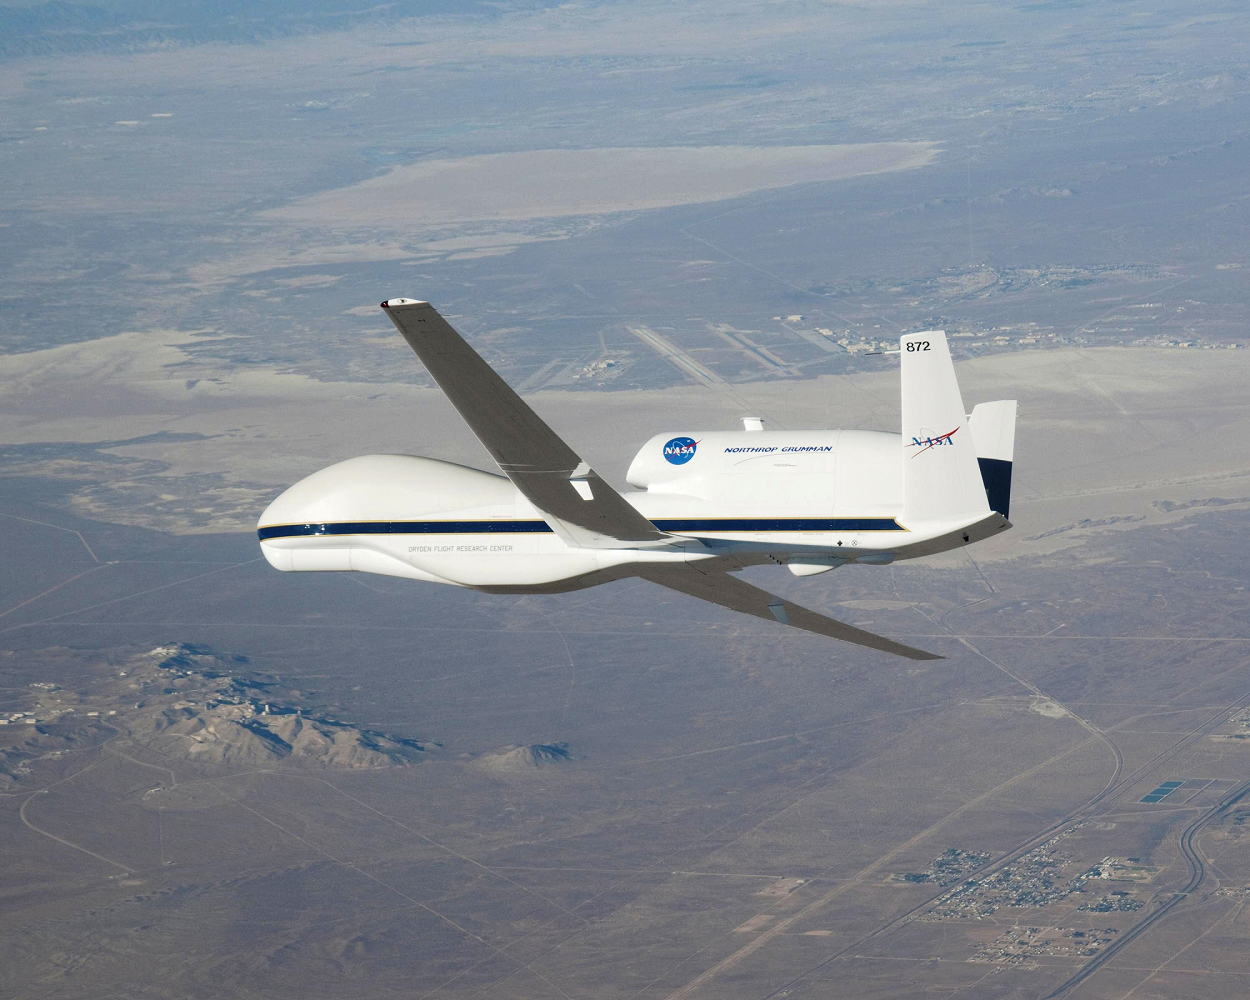
\includegraphics[width=\paperwidth,height=\paperheight]{Global-Hawk-NASA}
}

\usebackgroundtemplate{
}

\usebackgroundtemplate{
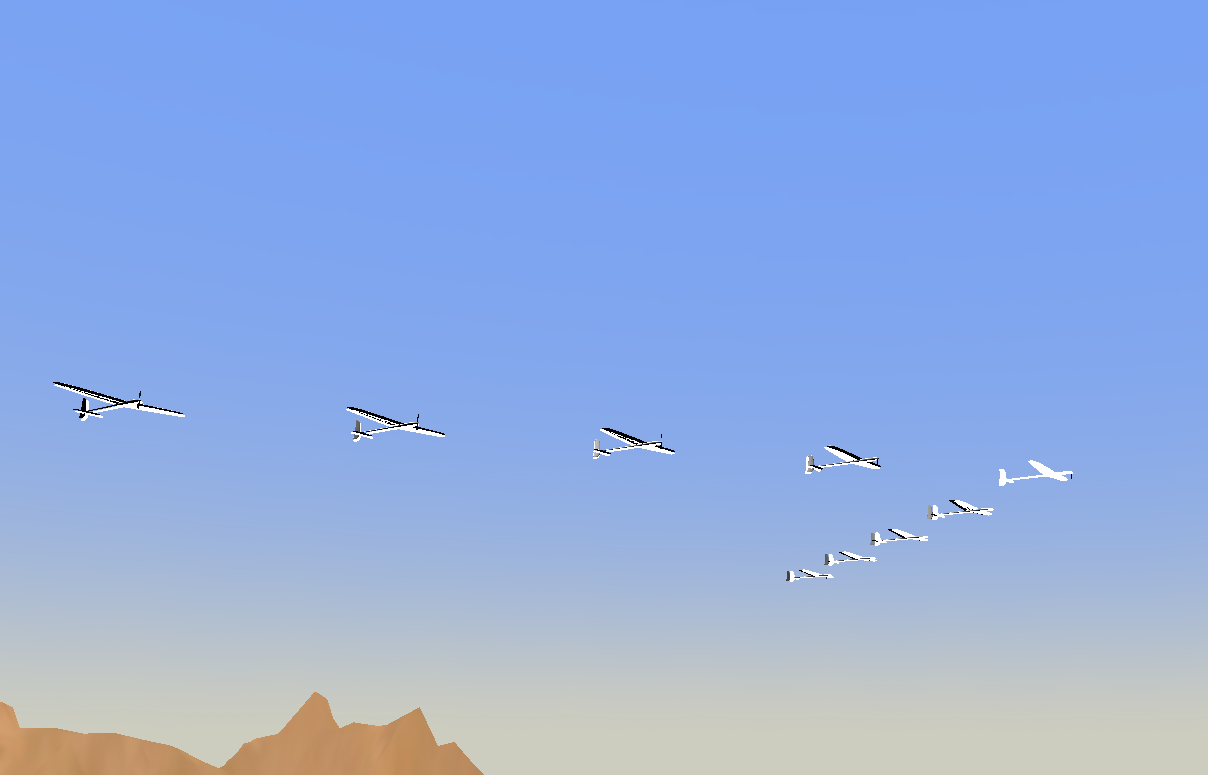
\includegraphics[width=\paperwidth,height=\paperheight]{dlg-9-II}
}

\begin{comment}
\begin{frame}{}
\vspace{-8em}
\centering
\begin{tcolorbox}[width=.8\textwidth,colback=gray!10!,title=Fleets of UAS]  
\centering
\begin{itemize}
\item Distributed payload
\item Enhanced endurance (order of Magnitude: 10-20 \%)
\item Limited hardware modifications
\end{itemize}
\centering
$\Rightarrow$ \textbf{(hopefully) less expensive}
\end{tcolorbox}  
\end{frame}
\end{comment}


\usebackgroundtemplate{} 
\begin{frame}{Benefit of tight and large formations \cite{Hummel1982}}
\begin{center}
\includegraphics[width=0.6\paperwidth]{Aerodynamic-graph-rouge}
\end{center}
\end{frame}

\begin{comment}
\usebackgroundtemplate{
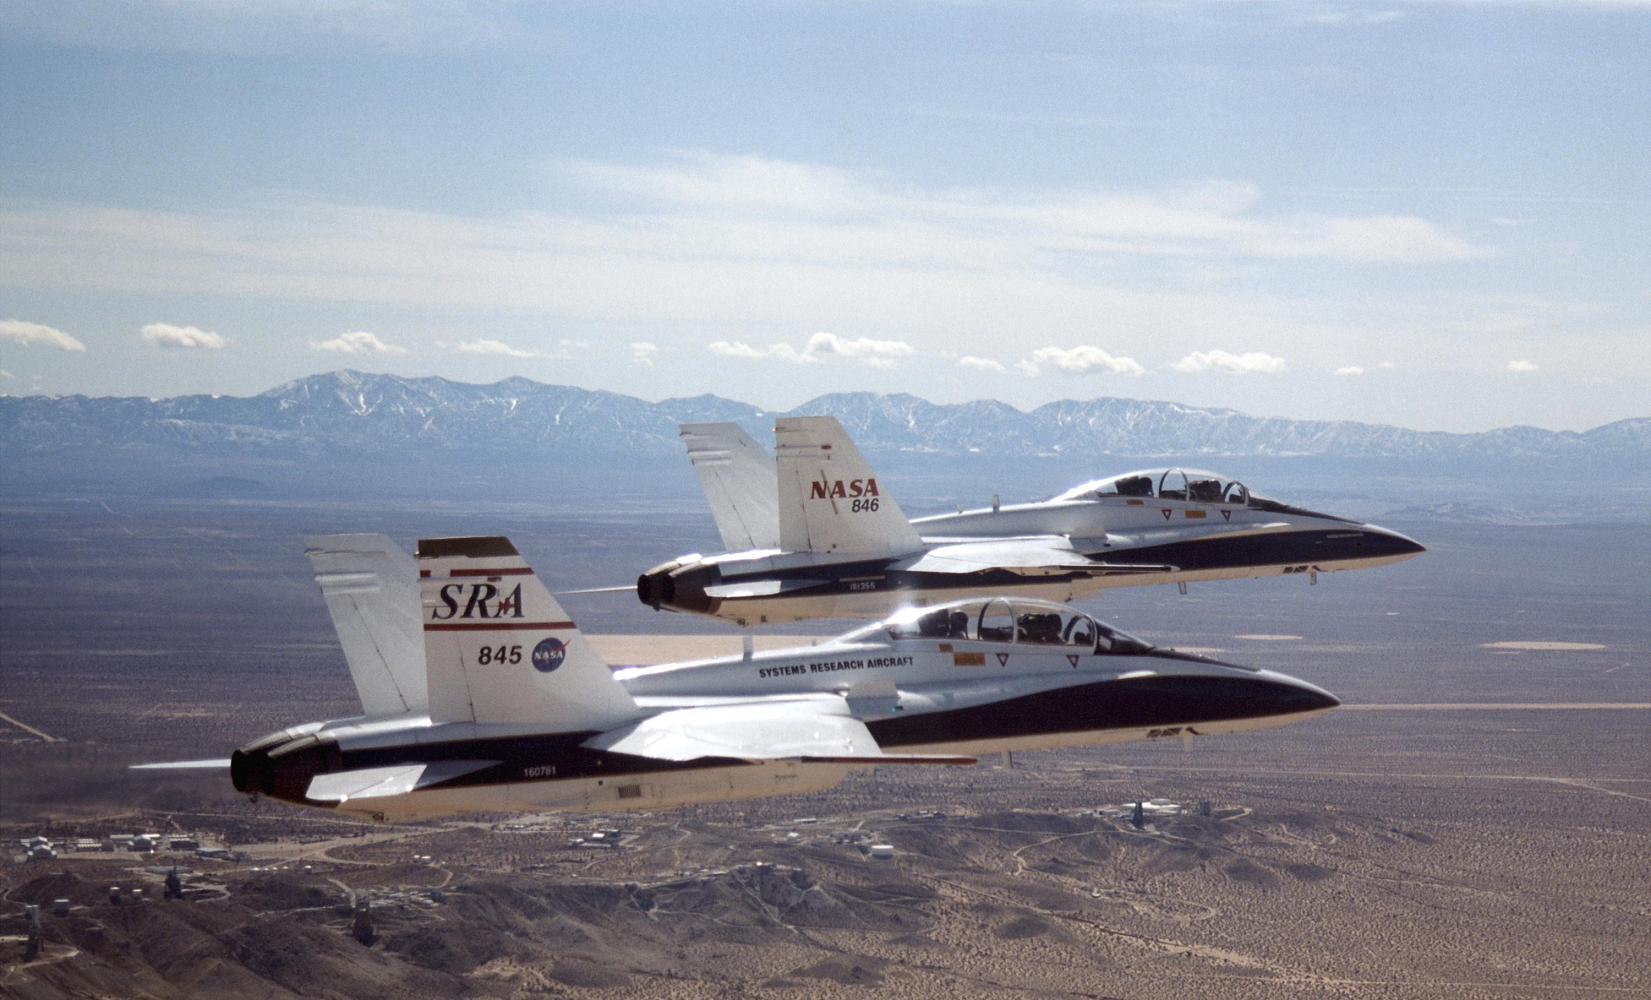
\includegraphics[width=\paperwidth,height=\paperheight]{NASA_AFF_1.png}
}
\begin{frame}{}

\vspace{-6em}
\centering

\begin{tcolorbox}[width=.8\textwidth,colback={gray!10!}]  
\centering
NASA \textbf{A}utonomus \textbf{F}ormation \textbf{F}light Program: \\
2x F-18 $\Rightarrow$ -18 \% fuel flow  \\
 $\Delta x$: peak fuel saving at $4.2 b$ downstream \cite{jake2003f}\\
 $-0.2 b < \Delta y < -0.1 b$ \\
 $-0.1 b < \Delta z < 0$ \\
  Linear control laws, not scalable
\end{tcolorbox}  

\end{frame}

\end{comment}

\begin{comment}
\usebackgroundtemplate{
\includegraphics[width=\paperwidth,height=\paperheight]{juppmehrbionik}
} 
\begin{frame}{Inspired by migratory birds}

\end{frame}

\end{comment}

\usebackgroundtemplate{
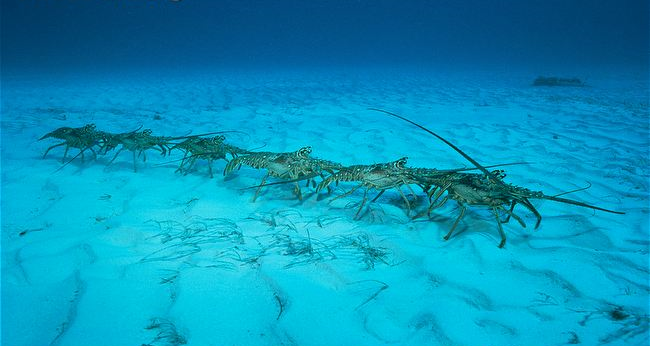
\includegraphics[width=\paperwidth,height=\paperheight]{lobsters}
}
\begin{frame}\frametitle{\textcolor{white}{Even lobsters do it}}
\end{frame}

\usebackgroundtemplate{
\includegraphics[width=\paperwidth,height=\paperheight]{juppmehrbionik}
} 

\begin{comment}
\begin{frame}\frametitle{\hspace{2em} Why is it hard for small UAS?}
\vspace{-1em}
\centering
\begin{tcolorbox}[width=.8\textwidth,colback={gray!10!}]  
\begin{itemize}
\item Heavy perturbations by vortices
\item Focus on guidance strategies in the community
\end{itemize}
\end{tcolorbox}  

\end{frame}
\end{comment}

\usebackgroundtemplate{}

\usebackgroundtemplate{
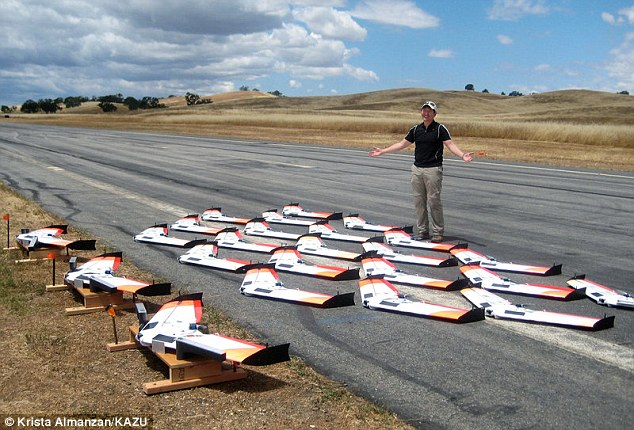
\includegraphics[width=\paperwidth,height=\paperheight]{ARSENL_swarm50}
}

\begin{frame}{Why is it hard?}
\centering
\vspace{-6em}
\begin{tcolorbox}[width=.99\textwidth,
colback={gray!10!},
standard jigsaw,
opacityback=1,  % this works only in combination with the key "standard jigsaw"
]  
\begin{itemize}
\item dm-level relative position control under heavy perturbations in the wake 
\item desirable property: only \textbf{local} relative state information
\item Existing linear control approaches (\cite{shaw2007controller}), require leader information for mesh stability
\end{itemize}
\end{tcolorbox}
\end{frame}

\usebackgroundtemplate{}
\begin{frame}
\centering
\Large
\vspace{3em}
\begin{center}
One promising candidate: \\
Sliding Mode Control\\
performance \& mesh stability
\end{center}
\end{frame}

\begin{frame}{Guidance level: system dynamics}
\centering
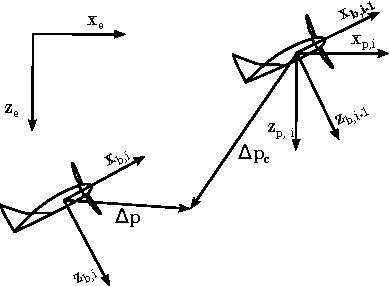
\includegraphics[width=4.4cm]{frames.pdf}    % The printed column width is 8.4 cm.
\begin{align}
\Delta \mbf{p}(t) &= \mbf{p}_\idxFollower(t) - \mbf{p}_\idxPredecessor(t) - \Delta \mbf{p}_c(t)  \nonumber \\
\Delta \dot{\mbf{p}}(t) &= \mbf{v}_{\idxFollower}(t) - \mbf{v}_{\idxPredecessor}(t) -  \Delta \dot{\mbf{p}}_c(t) \nonumber \\
\Delta \dot{\mbf{v}}(t) &= \mbf{a}_\idxFollower(t) - \mbf{a}_\idxPredecessor(t) -  \Delta \ddot{\mbf{p}}_c(t) \nonumber \\
{} &= \mbf{a}_{c,\idxFollower}(t) + \mbf{a}_{w,\idxFollower}(t)
 - \mbf{a}_\idxPredecessor(t) -  \Delta \ddot{\mbf{p}}_c(t) \nonumber \\
{} &= \mbf{u}(t) + \mbf{a}_{w,\idxFollower}(t)
 - \mbf{a}_\idxPredecessor(t) -  \Delta \ddot{\mbf{p}}_c(t) \nonumber
\end{align}
\end{frame}


\usebackgroundtemplate{
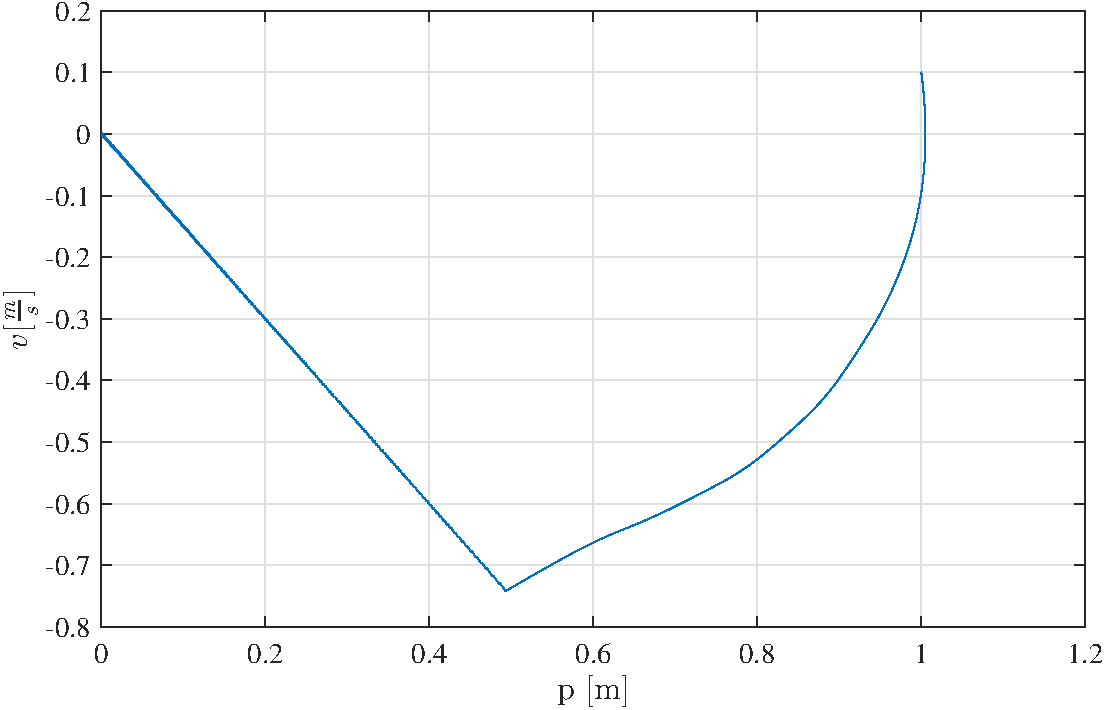
\includegraphics[width=\paperwidth,height=\paperheight]{smc-principle}
}

\begin{frame}\frametitle{}
\centering

\begin{tcolorbox}[colback=blue!5!white,colframe=blue!75!black,title=Ideal Sliding Mode Control, width=20em,
standard jigsaw,
opacityback=.7]
%\begin{tikzpicture}[remember picture, overlay]
%    \node[inner sep=0pt] at (6.3,-1.1) {%
%        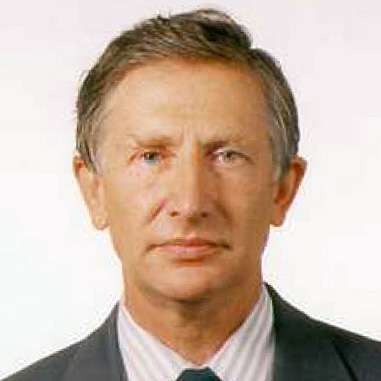
\includegraphics[width=.13\paperwidth]{utkin}%
%    };%
%\end{tikzpicture}
\begin{itemize}
\item Insensitive to \textbf{matched} perturbations
\item nonlinear
\item Recently proposed for platooning \cite{Fahimi2007} and formation flight \cite{galzi2006uav}
\end{itemize}
\end{tcolorbox}

\end{frame}

\usebackgroundtemplate{
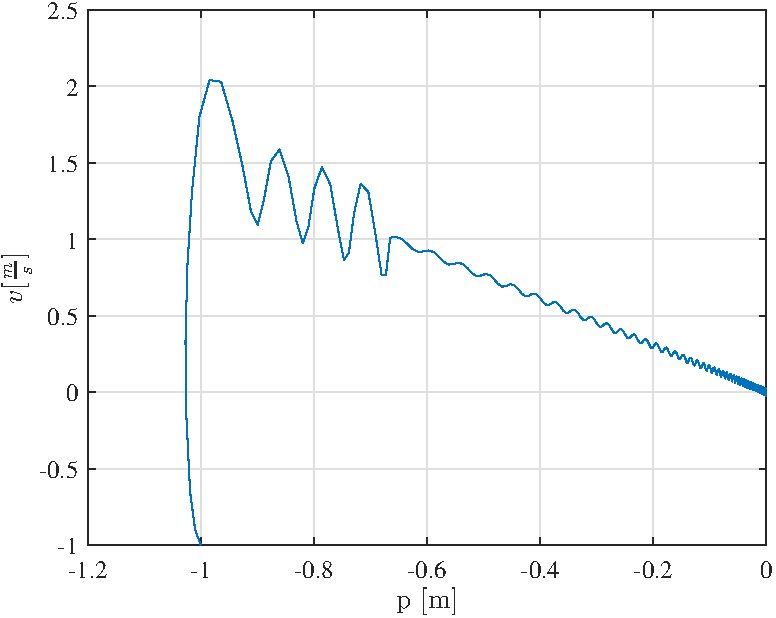
\includegraphics[width=\paperwidth,height=\paperheight]{smc-principle-chattering}
}
\begin{frame}\frametitle{}
\centering
\begin{tcolorbox}[colback=blue!5!white,colframe=blue!75!black,title=Clash with reality, width=20em,
standard jigsaw,
opacityback=.7]
\begin{itemize}
\item actuator dynamics $\Rightarrow$ perturbations unmatched 
\item delays
\item discrete implementation $\Rightarrow$ no infinite input switching
\end{itemize}
\centering
$\Rightarrow$ \textbf{ Chattering, loss of mesh stability} 
\end{tcolorbox}
\end{frame}

\usebackgroundtemplate{}
\begin{frame}
\Large
\vspace{3em}
\begin{center}
Continuous Time Sliding Mode Control applied to the UAS guidance loop
\end{center}
\end{frame}

\begin{comment}
\begin{frame}{Vortex perturbations: MHVM \cite{dogan2005modeling}}
\begin{center}
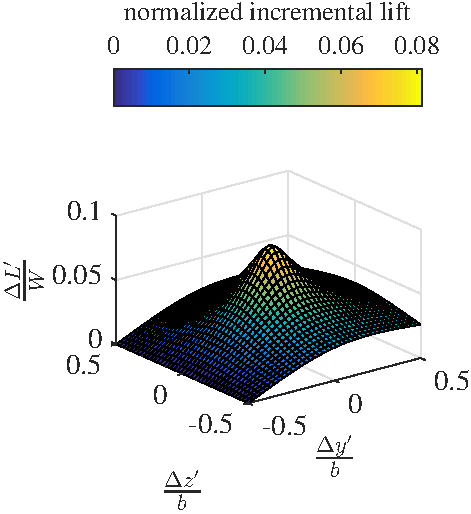
\includegraphics[height=.75\paperheight]{incrementallift.pdf}
\end{center} 
\end{frame}

\end{comment}
\begin{comment}
\begin{frame}{}
\centering
\Large
\vspace{3em}
Reference: \textbf{T}ime \textbf{S}ampled \textbf{C}ontinuous Higher Order \textbf{S}liding \textbf{M}ode \textbf{C}ontroller \cite{galzi2006uav} \\
\end{frame}

\end{comment}
\begin{frame}{Longitudinal: TSCSMC \cite{galzi2006uav} at 1000Hz}
\begin{center}
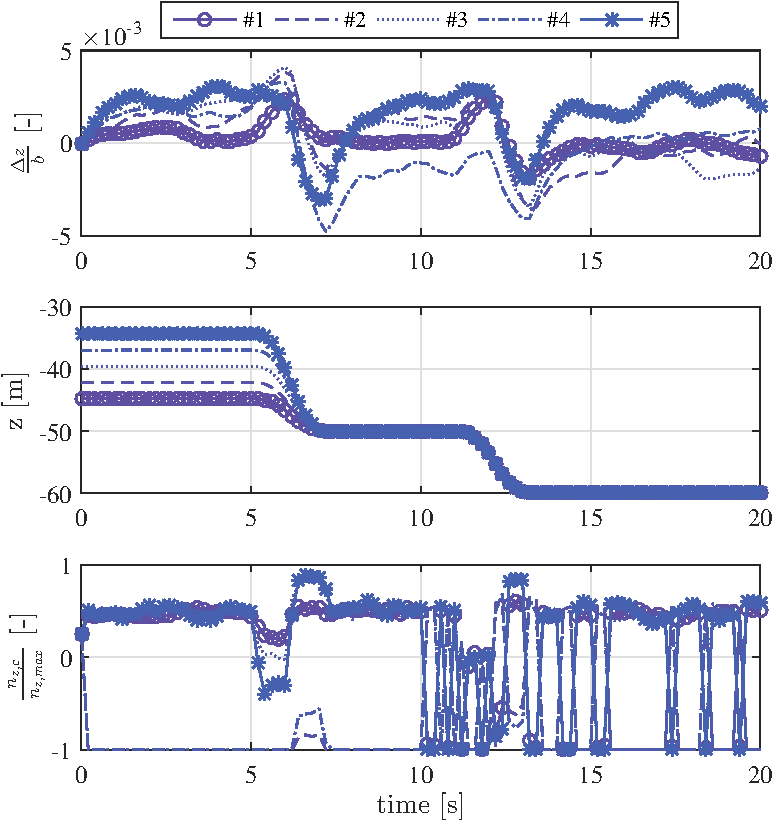
\includegraphics[height=.6\paperwidth]{TSCSMC-1000Hz-TIMESCALESEPARATION-turbulence=1}    
\end{center}% 
\end{frame}

\begin{frame}{Longitudinal: TSCSMC at 100Hz}
\begin{center}
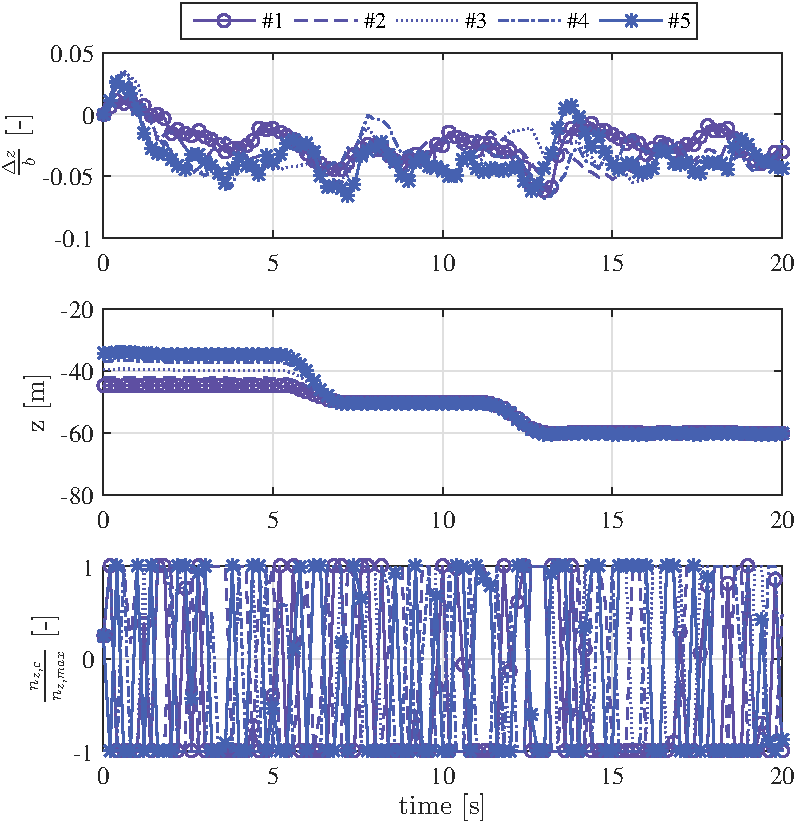
\includegraphics[height=.6\paperwidth]{TSCSMC-100Hz-TIMESCALESEPARATION-turbulence=1}    
\end{center}% 
\end{frame}

\usebackgroundtemplate{
}

\begin{frame}{Predictive Discrete Sliding Mode Control}
\centering
\begin{tcolorbox}[colback=blue!5!white,colframe=blue!75!black,title=PDSMC]
\begin{itemize}
\item Recent approach \cite{houda2013new}
\item Design directly in discrete time
\item Preserve spirit of Sliding Mode Control: stay in boundary layer of sliding surface
\item Minimizes boundary layer without tuning
\end{itemize}
\end{tcolorbox}
\end{frame}

\begin{frame}{Predictive Discrete Sliding Mode Control}
\centering
\begin{tcolorbox}[colback=blue!5!white,colframe=blue!75!black,title=What it looks like, width=.8\paperwidth]

\begin{align}
\mbf{\sigma}(\idxSample) &= \mbf{G}
\begin{pmatrix}
\Delta \mbf{p}(\idxSample)\\
\Delta \mbf{v}(\idxSample)
\end{pmatrix} \nonumber
\end{align}

\begin{align}
{{\sigma}}(\idxSample+1)
&=
{{\sigma}}(\idxSample)
+
T(
\mbf{\Phi}'_k(\idxSample) + \mbf{\Phi}'_u(\idxSample) + \mbf{u}(\idxSample))
\nonumber
\end{align}

\begin{align}
& \underset{\mbf{u}(\idxSample)}{\text{minimize}}
& & |\mbf{\sigma}(\idxSample+1)| \nonumber 
\end{align}

\end{tcolorbox}

\end{frame}

\begin{frame}{Predictive Discrete Sliding Mode Control}
\centering
\begin{tcolorbox}[colback=blue!5!white,colframe=blue!75!black,title=Adding hard magnitude and rate constraints \cite{Bolting2016}, width=.8\paperwidth]

\begin{align}
& \underset{\mbf{u}(\idxSample)}{\text{minimize}}
& & |\mbf{\sigma}(\idxSample+1)| \nonumber \\
& \text{subject to}
& & \mbf{U}_{min}(\idxSample) \leq \mbf{u}(\idxSample) \leq \mbf{U}_{max}(\idxSample) 
\nonumber
\end{align}

\begin{align}
|\mbf{u}(\idxSample) - \mbf{u}(\idxSample-1)| \leq \mbf{\Delta U} \nonumber
\end{align}

\begin{align}
\mbf{U}_{max}(\idxSample) = sat(\mbf{u}(\idxSample-1) + \mbf{\Delta U}, -\mbf{U}, \mbf{U}) \nonumber \\
\mbf{U}_{min}(\idxSample) = sat(\mbf{u}(\idxSample-1) - \mbf{\Delta U}, -\mbf{U}, \mbf{U}) \nonumber
\end{align}

\end{tcolorbox}
\end{frame}

\begin{comment}
\usebackgroundtemplate{}

\begin{frame}
\Large
\vspace{3em}

\begin{center}
Comparison \\to\\ discretized Continuous-time Sliding Mode Control (TSCSMC)
\end{center}
\end{frame}

\end{comment}
\begin{frame}{Simulation: PDSMC at 100Hz}
\begin{center}
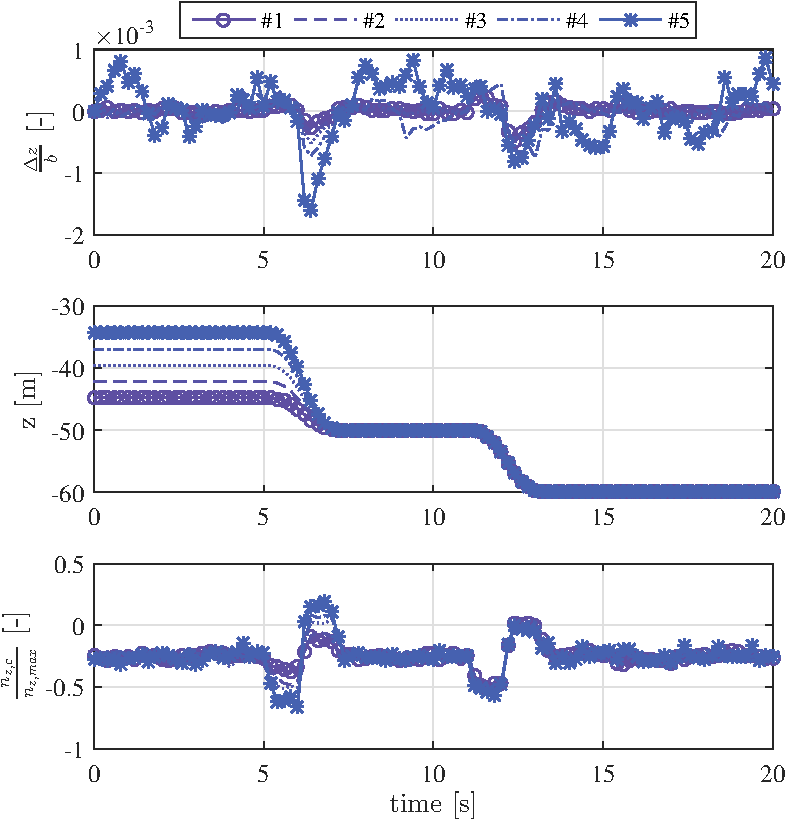
\includegraphics[height=.6\paperwidth]{PDSMC-100Hz-TIMESCALESEPARATION-turbulence=1}    % 

\end{center}\end{frame}

\begin{frame}{Figures of Merit vs. sampling time}

\begin{center}
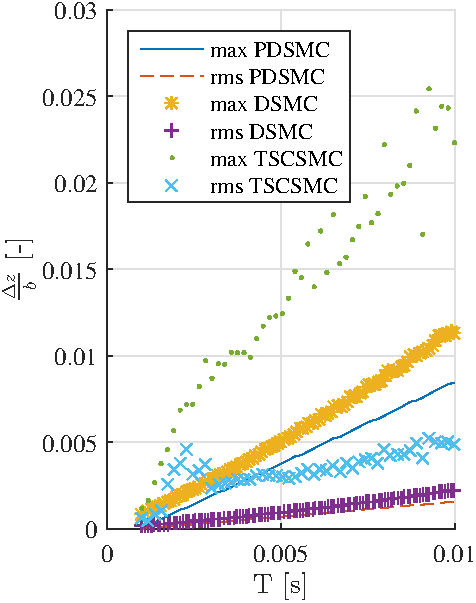
\includegraphics[height=0.8\paperheight]{error-z-vs-samplingtime.pdf}    

\end{center}\end{frame}

\begin{frame}{What about scalability?}
\centering
\begin{center}
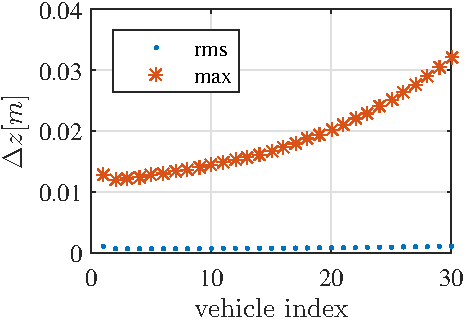
\includegraphics[width=\columnwidth]{erroramplification-DSMC-100Hz-TIMESCALESEPARATION-turbulence=1-turbulenceonlyfirstUAS} 

\end{center}\end{frame}

\begin{frame}{Conclusion \& Outlook}

\begin{tcolorbox}[width=.99\textwidth,
colback={blue!10!},
standard jigsaw,
opacityback=1,  % this works only in combination with the key "standard jigsaw"
]  
\begin{itemize}
\item PDSMC alleviates discretization issue of TSCSMC controller for TFF
\item Extends existing PDSMC approaches to respect inner loop constraints 
\end{itemize}
\end{tcolorbox}

\begin{tcolorbox}[width=.99\textwidth,
colback={red!10!},
standard jigsaw,
opacityback=1,  % this works only in combination with the key "standard jigsaw"
]  
\begin{itemize}
\item Extend PDSMC further: inner loop dynamics, lower sampling rates, observation noise
\item Better understand and quantify mesh instability
\end{itemize}
\end{tcolorbox}

\end{frame}

\usebackgroundtemplate{
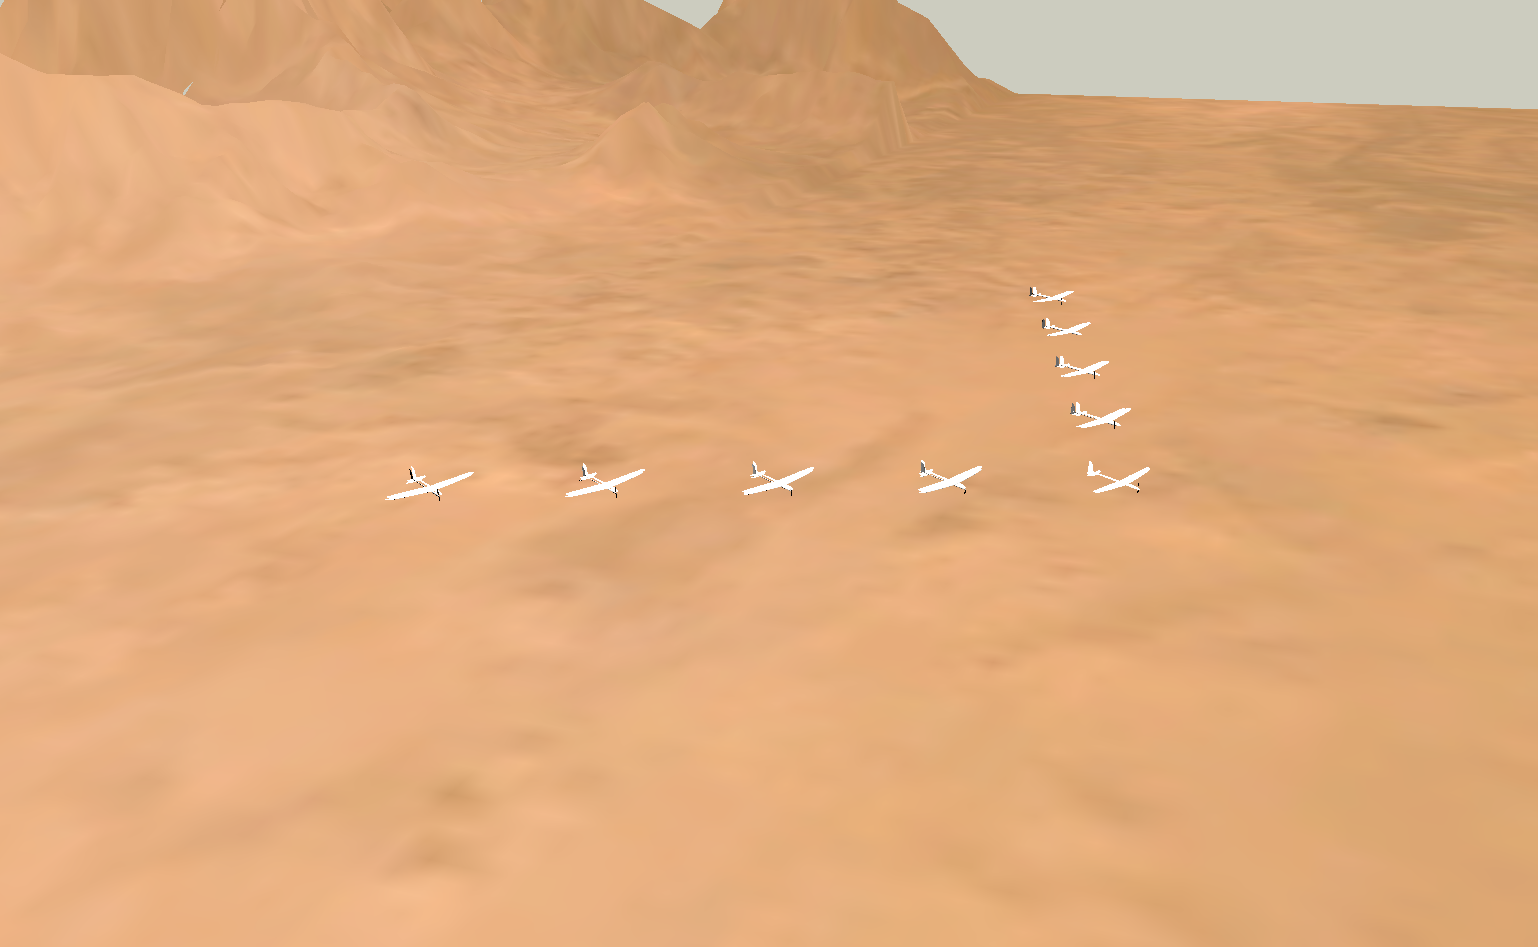
\includegraphics[width=\paperwidth,height=\paperheight]{dlg-9-2}
}

\begin{frame}
\end{frame}

\usebackgroundtemplate{}

\frametitle{References}

%\begin{frame}{References}
\bibliographystyle{ieeetr}
\bibliography{../../bibliography/bibliographyACA}        
%\bibliography{./../bibliography/bibliographyPhD}  
%\end{frame}

\end{document}
